\chapter{Το πρωτόκολλο LwM2M } % Main chapter title

\label{Chapter3} 

%\lhead{ΤΟ ΠΡΩΤΟΚΟΛΛΟ LWM2M} 

%%%%%%%%%%%%%%%%%%%%%%%%%%%% The paper headers

\section{Γενικά}
Το Lightweight M2M (\textbf{LwM2M}) αποτελεί ένα νέο, αναδυόμενο πρότυπο που αναπτύχθηκε από την Open Mobile Alliance (OMA) με μεγάλη συνάφεια με την αναπτυσσόμενη M2M βιομηχανία και το Διαδίκτυο των Αντικειμένων στο σύνολο του. Αυτό το βιομηχανικό πρότυπο παρέχει μέσα για την απομακρυσμένη διαχείριση μιας ευρείας γκάμας απομακρυσμένων ενσωματωμένων συσκευών και συνδεδεμένων συσκευών στο αναδυόμενο Διαδίκτυο των Αντικειμένων για την πραγματοποίηση εξ’ αποστάσεως εξυπηρέτησης και διαχείρισης απομακρυσμένων εφαρμογών [28].  

Η αγορά των διασυνδεδεμένων συσκευών αυξάνεται ρα­γδαία. Παρόλο που υπάρχουν βιομηχανικά πρότυπα διαθέσιμα που ικανοποιούν τις απαιτήσεις απομακρυσμένης διαχείρισης, για παράδειγμα σταθερών ευρυζωνικών δρομολογητών και smartphones, αυτά τα καθιερωμένα πρότυπα δεν είναι ιδιαίτερα χρήσιμα για την απομακρυσμένη διαχείριση μιας μεγάλης και ανα­πτυσσόμενης κατηγορίας συνδεδεμένων συσκευών: εκείνων με περιορισμένο εύρος ζώνης δικτύου, υπολογιστικής ισχύος και μνήμης, εκείνων που εξαρτώνται από περιορισμένη διάρκεια ζωής της μπαταρίας και εκείνων που είναι βιώσιμα μόνο με πολύ χαμη­λό κόστος παραγωγής. Ως εκ τούτου, αναλήφθηκε αυτή η νέα προ­σπάθεια για τη δημιουργία ενός μηχανισμού που να καλύπτει επίσης τις ανάγκες των “περιορισμένων” συσκευών. Η βιομηχα­νία αναζητά έναν απλό, χαμηλού κόστους απομακρυσμένο μηχανι­σμό διαχείρισης και ενεργοποίησης υπηρεσιών, ο οποίος να περιλαμβάνει σύγχρονες αρχιτεκτονικές αρχές (σύμφωνα με τα πρότυ­πα του Διαδικτύου) ενώ παράλληλα να λειτουργεί μέσω ασύρμα­των συνδέσεων και να είναι κατάλληλος για το σκοπό αυτό λόγω των χαμηλών απαιτήσεων σε πόρους. Τη λύση έρχεται να δώσει το πρωτόκολλο LwM2M.

Από τεχνικής άποψης, το LwM2M πρόκειται για ένα πρωτόκολλο επικοινωνίας για χρήση μεταξύ του λογισμικού του client μιας M2M συσκευής και του λογισμικού του server σε μια πλατφόρμα διαχείρισης και ενεργοποίησης υπηρεσιών Μ2Μ. Το πρωτόκολλο LwM2M που χρησιμοποιείται για την απομακρυσμένη διαχείριση Μ2Μ συσκευών και τις σχετικές δυνατότητες εξυπηρέτησης έχει τέσσερα εξαιρετικά χαρακτηριστικά [28]:

\begin{enumerate}
	\item{Διαθέτει σύγχρονο αρχιτεκτονικό σχεδιασμό βασι­σμένο στο REST που απευθύνεται σε προγραμματιστές.}
	\item{Ορίζει ένα μοντέλο πόρων και δεδομένων.}
	\item{Έχει σχεδιαστεί με γνώμονα την απόδοση και τους περιορισμένους πόρους των συσκευών Μ2Μ.}
	\item{Επαναχρησιμοποιείται και βασίζεται σε ένα αποδοτικό πρότυπο μεταφοράς δεδομένων, το CoAP που περιγράφηκε παραπάνω.}
\end{enumerate}

Η διαθεσιμότητα αυτού του ανοικτού κώδικα, τυποποιη­μένου μηχανισμού απομακρυσμένης διαχείρισης δημιουργεί τις ακόλουθες ευκαιρίες και επιχειρηματικά οφέλη για τους διάφο­ρους “παίκτες” της βιομηχανίας Μ2Μ [28]:

\begin{itemize}
	\item{Θα μειώσει τον βαθμό κατακερματισμού (fragmentation) στον τομέα της απομακρυσμένης διαχείρισης συσκευών M2Μ, επιτρέποντας έτσι περισσότερες plug-n-play λύσεις μεταξύ μιας αυξανόμενης ποικιλίας συσκευών Μ2Μ και των πλατφορμών διαχείρισης τους.}
	\item{Δεδομένου του σχεδιασμού του για την κάλυψη των περιορισμένων συσκευών, μπορεί να λειτουργήσει ως ένας παράγοντας που διευκολύνει την ανάπτυξη της αγοράς Μ2Μ σε διάφορους τομείς, από την διαχείριση μίας “έξυπνης” πόλης μέχρι την διαχείριση ενέργειας και την παρακολούθηση θέσης. Πιο συγκεκριμένα θα ωφεληθούν τομείς όπου οι συσκευές πρέπει να έχουν χαμηλό κόστος για να καταστήσουν δυνατή την ανάπτυξη βιώσιμων επιχειρηματικών μοντέλων.}
	\item{Αυτό το νέο πρότυπο θα μπορούσε να βελτιώσει σημαντικά τον χρόνο time-to-market και την διαχειρισιμότητα των συσκευών, παρέχοντας για  πρώτη φορά μια λύση που μπορεί να χρησιμοποιηθεί τόσο για την διαχείριση συσκευών όσο και για εφαρμογές δεδομένων και υπηρεσιών, ανεξάρτητα από το πως φιλοξενούνται τα στοιχεία του συστήματος.}
	\item{Ως πρωτόκολλο απομακρυσμένης διαχείρισης μεταξύ συσκευών και πλατφορμών Μ2Μ οδηγεί σε αποσύνδεση και των δύο πλευρών, επιτρέποντας έτσι μεγαλύτερη ανεξάρτητη καινοτομία των συσκευών Μ2Μ και των πλατφορμών Μ2Μ. }
\end{itemize}

\section{Περιγραφή των μηχανισμών του LwM2M}
Το LwM2M είναι βασισμένο και σχεδιασμένο πάνω στο CoAP και χρησιμοποιεί προαιρετικά το πρωτόκολλο DTLS για την ανάπτυξη εφαρμογών που απαιτούν ασφαλή επικοινωνία. Στην ει­κόνα 3.1 δίνεται μία οπτικοποίηση της αρχιτεκτονικής του LwM2M πρωτοκόλλου. Μια προς διαχείριση συσκευή αποτελεί έναν LwM2M client ενώ η πλατφόρμα διαχείρισης της συσκευής είναι ένας LwM2M server. Για την επικοινωνία μεταξύ αυτών των δύο το LwM2M ορίζει τέσσερα interfaces που είναι τα εξής:

\begin{enumerate}
	\item{\textbf{Bootstrap}: ορίζει την διαδικασία που απαιτείται ώστε ένας LwM2M client να λάβει τις απαιτούμενες πληροφορίες για τον server στον οποίο πρέπει να συνδεθεί (register).}
	\item{\textbf{Client Registration}: ορίζει την απαιτούμενη διαδικασία κατά την οποία ένας client εγγράφεται ή απεγγράφεται από έναν LwM2M server.}
	\item{\textbf{Device Management and Service Enablement}:  περιγράφει τον τρόπο με τον οποίο ένας LwM2M server προσπελαύνει τα LwM2M objects και τα LwM2M resources που έχει ένας LwM2M client.}
	\item{\textbf{Information Reporting}: χρησιμοποιείται από τον server για την παρακολούθηση αλλαγών σε κάποιο resource του client.}
\end{enumerate}

Ο client αλληλεπιδρά με τον server ακολουθώντας τις αρχές της REST αρχιτεκτονικής. Κάθε υπηρεσία ή πληροφορία που διαθέτει ένας LwM2M client στο περιβάλλον του αποτελεί ένα LwM2M resource. Κάθε resource μεταξύ των υπόλοιπων ιδιοτήτων του, χαρακτηρίζεται και από έναν τύπο (type). Ένα resource μπορεί να είναι τύπου {String, Float, Integer, Boolean, Opaque, Time, ObjLink}. Τα resources είναι λογικά ομαδοποιημένα σε LwM2M Objects. Ένας LwM2M client μπορεί να έχει οποιοδήποτε αριθμό από resources τα οποία όμως ανήκουν σε κάποιο object. Κάθε object μπορεί να έχει ένα μοναδικό ή πολλαπλά στιγμιότυπα (object instances).


\begin{figure}[htbp]
	\centering
		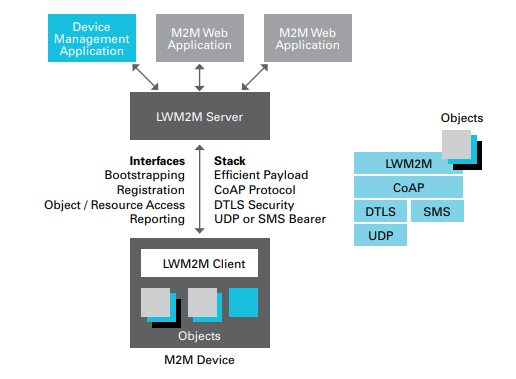
\includegraphics[height=10cm,width=15cm]{Figures/5.png}
	\caption{Η LwM2M αρχιτεκτονική \cite{OMA1} }	
\end{figure}

Κάθε {object/ object instance /resource ενός συγκεκριμένου object} αναγνωρίζεται μονοσήμαντα από ένα μοναδικό {object id/ object instance id / resource id} αντίστοιχα. Η αναφορά σε κάποιο resource γίνεται μέσα από ένα path με τη μορφή “/{Object ID}/{Object Instance ID}/{Resource ID}”. 
	
Ο LwM2M server όταν θέλει να ξεκινήσει μία αλληλεπίδραση με έναν LwM2M client του αποστέλλει ένα αίτημα. Ένα τέτοιο αίτημα απαρτίζεται από το path του resource στο οποίο αναφέρεται και την μέθοδο την οποία αιτείται να εφαρμοστεί στο resource αυτό. 	Το Device Management \& Service Enablement Interface (DM\&SE) ορίζει το σύνολο των μεθόδων που \textbf{πρέπει} να υποστηρίζει τόσο ένας LwM2M client όσο και ο LwM2M server και μπορούν να εφαρμοστούν σε ένα resource [32]. Αυτές είναι:
	
\begin{enumerate}
	\item{\textbf{CREATE}: Δημιουργεί instance}
	\item{\textbf{READ}: Ζητείται να επιστραφεί η τιμή ενός resource}
	\item{\textbf{WRITE}: Ζητείται η αλλαγή της τιμής ενός resource}
	\item{\textbf{DELETE}: Διαγραφεί instance}
	\item{\textbf{EXECUTE}: Ζητείται η πραγματοποίηση μίας ενέργειας}
	\item{\textbf{WRITE-ATTRIBUTES}: Χρησιμοποιείται για την αλλαγή των τιμών των attributes}
	\item{\textbf{DISCOVER}: Χρησιμοποιείται για την ανακάλυψη resources και attributes}
\end{enumerate}

Αφού ο LwM2M server αποστείλει το αίτημα ο LwM2M client στέλνει πίσω μία απάντηση η οποία περιέχει έναν κωδικό απάντησης και σε κάποιες περιπτώσεις ένα περιεχόμενο. Για παράδειγμα μια απάντηση σε ένα αίτημα READ μπορεί να έχει για κωδικό απάντησης το “2.04 Changed” και για περιεχόμενο την τιμή του resource το οποίο αφορούσε το αίτημα. Ανάλογα τον τύπο του αρχικού αιτήματος, ο κωδικός απάντησης έχει διαφορετική σημασία [32].	

	Μεγάλη σημασία έχει επίσης και ο μηχανισμός observe του CoAP, ο οποίος χρησιμοποιείται από το LwM2M μέσω του Information Reporting Interface. Αυτό το interface χρησιμοποιείται από έναν LwM2M server ώστε να παρατηρούνται οι αλλαγές που γίνονται σε ένα resource ενός καταχωρημένου LwM2M client. Κάθε φορά που αλλάζει η τιμή του resource αποστέλλεται μία ειδοποίηση στον LwM2M server μαζί με τη νέα τιμή του resource. Αυτή η σχέση observe-notify ξεκινά με την αποστολή ενός αιτήματος τύπου “observe”  από τον server στον client για ένα object, object instance ή resource που είναι παρακολουθήσιμο (observable).Μετά από την επιτυχή εγκαθίδρυση μιας τέτοιας σχέσης, ο LwM2M client αποστέλλει ένα μήνυμα τύπου “notify” στον server. Το μήνυμα αυτό περιέχει τη νέα τιμή του resource που παρακολουθείται. Η εικόνα 3.2 δείχνει το μοντέλο λειτουργίας για το συγκεκριμένο interface:

\begin{figure}[htbp]
	\centering
		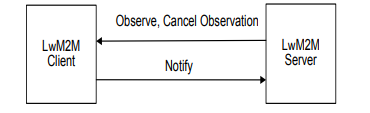
\includegraphics[height=3cm,width=9cm]{Figures/6.png}
	\caption{LwM2M Information Reporting Interface \cite{OMA2} }	
\end{figure}

Αξίζει να σημειωθεί ότι ο οργανισμός ΟΜΑ μαζί με τις προδιαγραφές του LwM2M δημοσιοποιεί και ένα μητρώο (registry) το οποίο περιέχει όλα τα LwM2M objects τα οποία έχουν καταχωρηθεί σε αυτό από τον οργανισμό καθώς και από τρίτους. Αυτό το μητρώο υλοποιήθηκε με στόχο ένας LwM2M client να μπορεί να ενημερώσει έναν LwM2M server για τα objects τα οποία μπορεί να υποστηρίξει αποστέλλοντας μόνο το object ID. Έτσι όλα τα χαρακτηριστικά καθώς και τα resources που αφορούν τα objects αυτά μπορούν να ανασυρθούν από αυτό το μητρώο που μπορεί να βρίσκεται είτε τοπικά στην μνήμη του LwM2M server είτε στο Διαδίκτυο. Επιπρόσθετα έχει υλοποιηθεί και άλλο ένα μητρώο το Resource Registry το οποίο περιέχει επαναχρησιμοποιούμενα resources τα οποία έχουν κοινά χαρακτηριστικά και σημασία για κάθε LwM2M object που τα χρησιμοποιεί. Στην συγκεκριμένη εργασία δημιουργήθηκε ένα μητρώο που βρίσκεται τοπικά στην μνήμη του LwM2M server.

	Επειδή η παρούσα εργασία αφορά την υλοποίηση του Industrial Automation Thing δεν δόθηκε ιδιαίτερη έμφαση στην υλοποίηση του LwM2M server. Εν αντιθέσει υλοποιήθηκε ο LwM2M client ώστε να χρησιμοποιηθούν τα πλεονεκτήματα που δίνονται από το LwM2M. Ο LwM2M server που χρησιμοποιήθηκε υλοποιήθηκε σε άλλη διπλωματική εργασία που εκπονήθηκε ταυτόχρονα με την παρούσα. 
	
\section{Πλεονεκτήματα του  LwM2M}

Το πρωτόκολλο LwM2M επιλύει ένα σύνολο τεχνολογικών προκλήσεων που σχετίζονται με την διαχείριση συσκευών και την ενεργοποίηση end-to-end υπηρεσιών καθώς η αγορά M2M ωριμάζει και το Διαδίκτυο των Αντικειμένων καθιστούν εφικτή την επικοινωνία μεταξύ τέτοιων συσκευών. Παρακάτω συνοψίζονται τα οφέλη που παρέχει το LwM2M [28]: 

\begin{itemize}
	\item{Μεγαλύτερη ανάπτυξη της αγοράς και αποδοτικότητα κόστους για ολόκληρη την βιομηχανία,  μέσω των τεχνολογιών που προσφέρει το LwM2M οι οποίες καθιστούν εφικτή την χαλαρή σύνδεση συσκευών, την εύκολη διαχείριση τους και την διαχείριση των υπηρεσιών που αυτές προσφέρουν.}
	\item{Οι πάροχοι υπηρεσιών, οι OEMs και οι τελικοί χρήστες επωφελούνται από την ομοιόμορφη διαχείριση των διάφορων συσκευών.}
	\item{Σε σύγκριση με τις protocol stacks που χρησιμοποιούνται στις παραδοσιακές συσκευές, το LwM2M μπορεί να παρέχει 10x αύξηση της αποδοτικότητας.}
	\item{Το LwM2M συμπληρώνει τις υπάρχουσες λύσεις διαχείρισης συσκευών, όπως το ΟΜΑ DM και το Broadband Forum TR-69, και επεκτείνει σε μεγάλο βαθμό το εύρος των συσκευών που μπορούν να διαχειριστούν με ασφάλεια.}
	\item{Το μοντέλο δεδομένων του LwM2M καθώς και το μητρώο των αντικειμένων παρέχουν προσβάσιμη και επαναχρησιμοποιήσιμη σημασιολογία τόσο για την διαχείριση συσκευών όσο και για την διαχείριση των δεδομένων μιας εφαρμογής για όλο το Διαδίκτυο των Αντικειμένων στην βιομηχανία. }
	\item{Παρέχοντας μια ενιαία λύση για την διαχείριση των συσκευών και των δεδομένων τους το LwM2M απλοποιεί τα διάφορα συστήματα και επιτρέπει την δημιουργία νέων και καινοτόμων υπηρεσιών M2M.}
	\item{Η πλήρης διαχείριση του κύκλου ζωής και της ασφάλειας που είναι κατάλληλη για περιορισμένες συσκευές επιλύει ένα από τα πιο πιεστικά προβλήματα στη βιομηχανία M2M.}
	\item{Το LwM2M ορίζει μόνο της διεπαφή δικτύου της συσκευής, επιτρέποντας έτσι την εύκολη ενσωμάτωση του σε υπάρχουσες υπηρεσίες διαχείρισης συσκευών και υπηρεσιών Μ2Μ.}
\end{itemize}




